% Created 2024-04-23 Tue 15:30
% Intended LaTeX compiler: pdflatex
\documentclass[presentation]{beamer}
\usepackage[utf8]{inputenc}
\usepackage[T1]{fontenc}
\usepackage{graphicx}
\usepackage{longtable}
\usepackage{wrapfig}
\usepackage{rotating}
\usepackage[normalem]{ulem}
\usepackage{amsmath}
\usepackage{amssymb}
\usepackage{capt-of}
\usepackage{hyperref}
\mode<beamer>{\usetheme{Madrid}}
\definecolor{SUred}{rgb}{0.59375, 0, 0.17969} % SU red (primary)
\definecolor{SUblue}{rgb}{0, 0.17578, 0.38281} % SU blue (secondary)
\setbeamercolor{palette primary}{bg=SUred,fg=white}
\setbeamercolor{palette secondary}{bg=SUblue,fg=white}
\setbeamercolor{palette tertiary}{bg=SUblue,fg=white}
\setbeamercolor{palette quaternary}{bg=SUblue,fg=white}
\setbeamercolor{structure}{fg=SUblue} % itemize, enumerate, etc
\setbeamercolor{section in toc}{fg=SUblue} % TOC sections
% Override palette coloring with secondary
\setbeamercolor{subsection in head/foot}{bg=SUblue,fg=white}
\setbeamercolor{date in head/foot}{bg=SUblue,fg=white}
\institute[SU]{Shenandoah University}
\titlegraphic{
\includegraphics[width=0.5\textwidth]{\string~/Documents/suLogo/suLogo.pdf}}
\newcommand{\R}{\mathbb{R}}
\usepackage{tikz}
\usepackage{pgfplots}
\usetheme{default}
\author{Chase Mathison\thanks{cmathiso@su.edu}}
\date{24 April 2024}
\title{Properties of Power Series}
\hypersetup{
 pdfauthor={Chase Mathison},
 pdftitle={Properties of Power Series},
 pdfkeywords={},
 pdfsubject={},
 pdfcreator={Emacs 29.1 (Org mode 9.6.7)}, 
 pdflang={English}}
\begin{document}

\maketitle

\section{Announcements}
\label{sec:org5b14a36}
\begin{frame}[label={sec:org5dc63a9}]{Announcements}
\begin{enumerate}
\item Homework in MyOpenMath.
\item Exam next Wednesday.
\item Office hours, 10am - 11am.
\end{enumerate}
\end{frame}

\section{Warm up problem}
\label{sec:orgdc311cb}
\begin{frame}[label={sec:orgd24411d}]{Warm up problem}
What is the limit of the following recursively defined sequence?
\[
x_{n+1}  = x_n - 1 + 2e^{-x_n}, x_0 = 1.\]
\vspace{10in}
\end{frame}

\section{Properties of power series}
\label{sec:orga7ef826}
\begin{frame}[label={sec:org57cf7e8}]{Properties of Power Series}
To find power series representations of other functions,
it's going to be convenient to combine power series that we already know

\begin{center}
\begin{center}
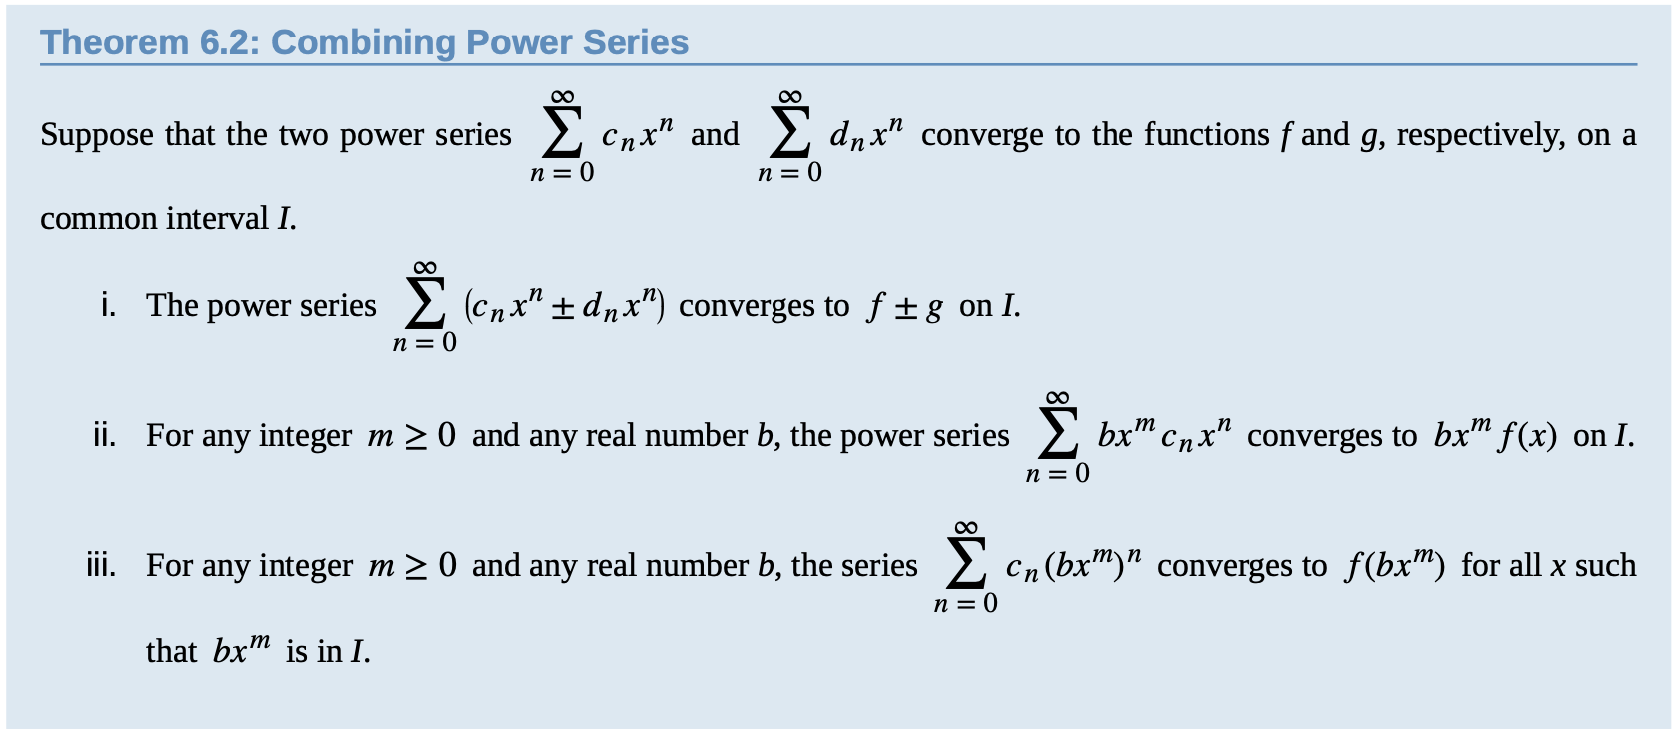
\includegraphics[width=.9\linewidth]{../img/combiningPowSer.png}
\end{center}
\end{center}
\end{frame}

\begin{frame}[label={sec:org7b9bcc1}]{Example}
Find a power series representation centered at 0 for the function
\[f(x) = \frac{x}{1 + x^2}.\]
\vspace{10in}
\end{frame}

\begin{frame}[label={sec:org6363580}]{Example}
\end{frame}

\begin{frame}[label={sec:orgcb4d7cf}]{Example}
Use the geometric series to find a power series centered at \(a = 2\)
for the function \[\frac{1}{\left( x-1 \right)\left( x-3 \right)}\]

\vspace{10in}
\end{frame}

\begin{frame}[label={sec:org6e981b4}]{Example}
\end{frame}

\begin{frame}[label={sec:org8211792}]{Differentiation and integration of power series}
\begin{center}
\begin{center}
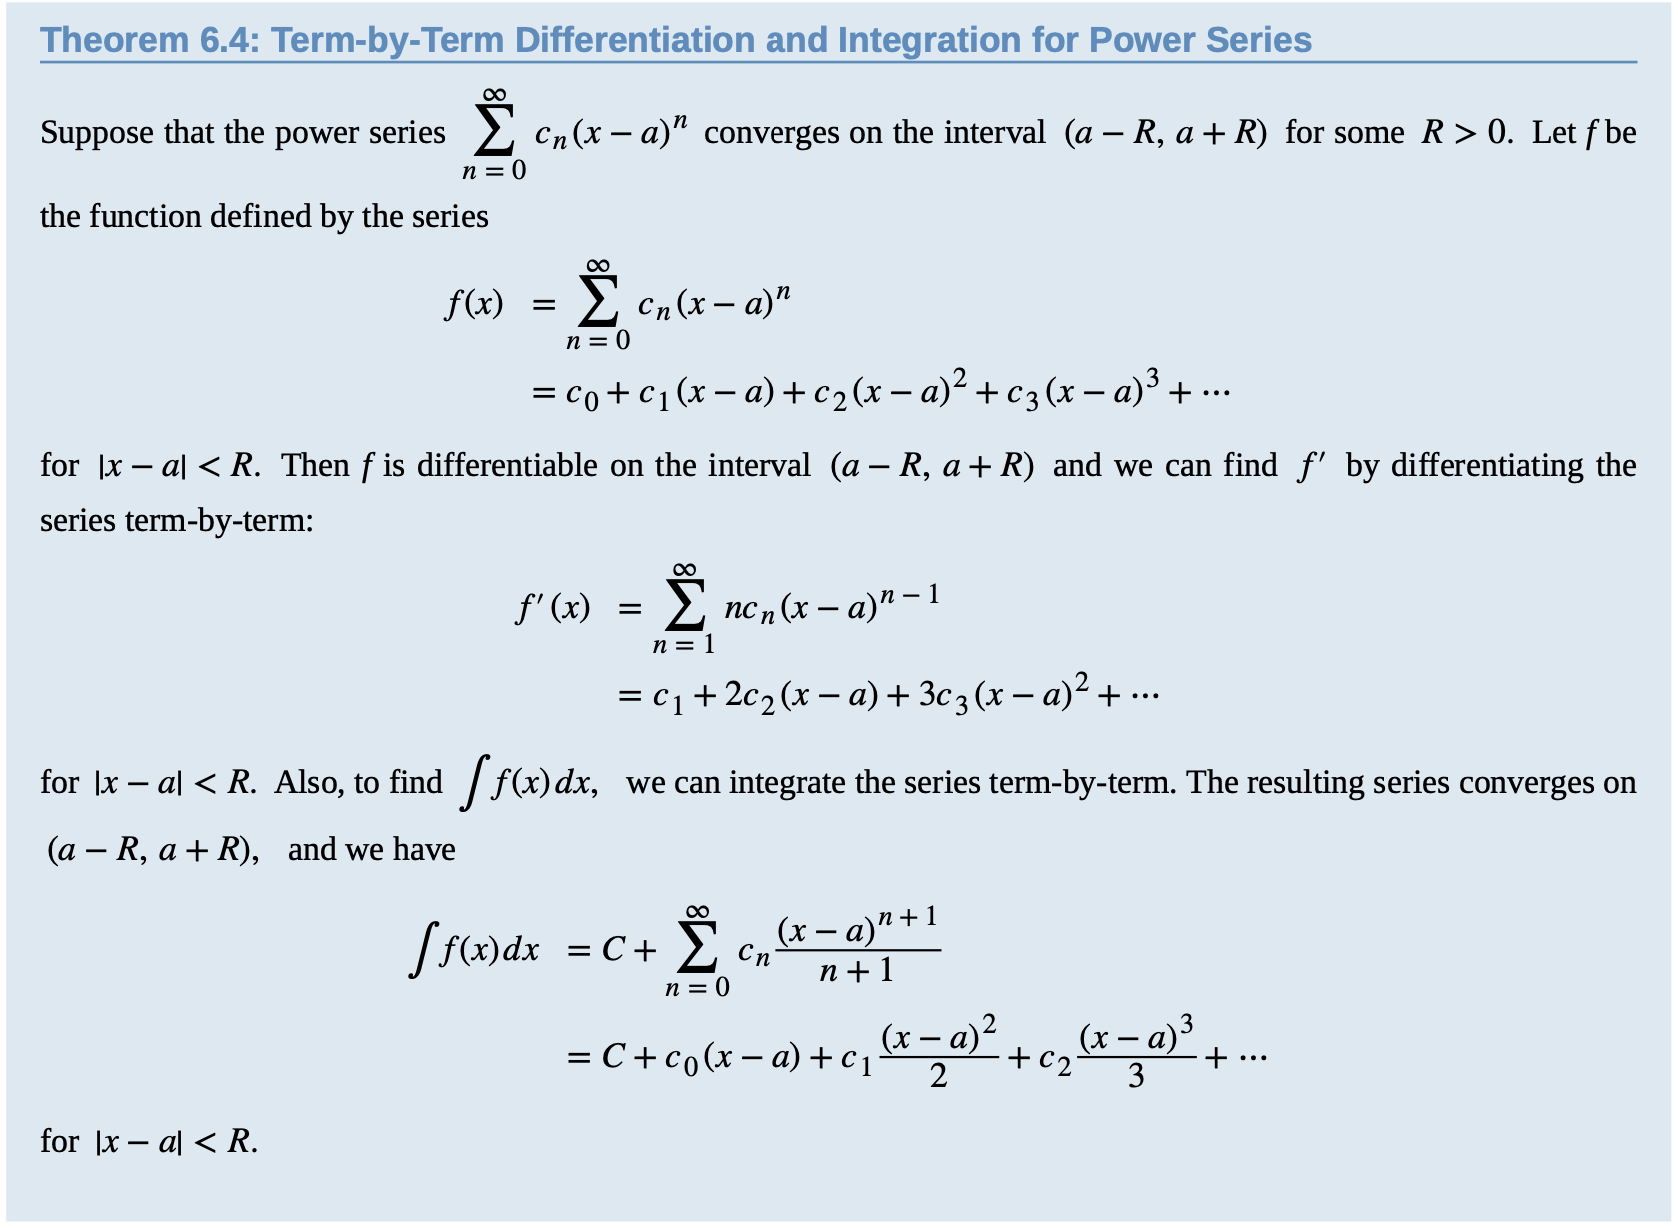
\includegraphics[width=.9\linewidth]{../img/tbyt.png}
\end{center}
\end{center}
\end{frame}

\begin{frame}[label={sec:orgc1c3ee4}]{Differentiation and integration of power series}
Note that this theorem says \(f(x)\) and \(f'(x)\) have the same
radius of convergence, but does NOT tell us if they have the same
endpoint behavior. The same goes for integrals.
\end{frame}

\begin{frame}[label={sec:orga0639e1}]{Example}
Find a power series representation centered at 0 for

\begin{enumerate}
\item \(\frac{2x}{1-x^2}\)

\item \(\ln(1+x)\)

\item \(\arctan(x)\)
\vspace{10in}
\end{enumerate}
\end{frame}

\begin{frame}[label={sec:org4162815}]{Uniqueness}
One last point to note is that power series representations
are \uline{\hspace*{1in}}.

\begin{center}
\begin{center}
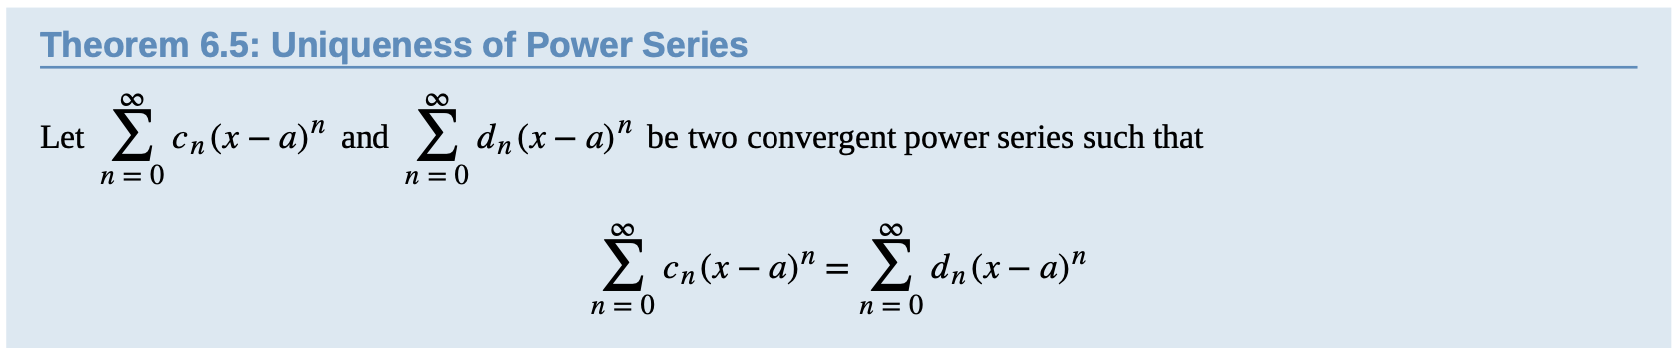
\includegraphics[width=.9\linewidth]{../img/unique1.png}
\end{center}

\begin{center}

\includegraphics[width=.9\linewidth]{../img/unique2.png}
\end{center}
\end{center}

\emph{Proof:}
\vspace{10in}
\end{frame}

\begin{frame}[label={sec:org06c6229}]{Example}
\begin{center}
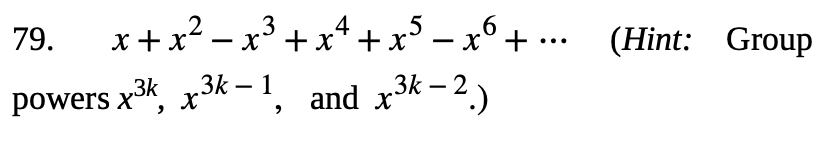
\includegraphics[width=.9\linewidth]{../img/prob1.png}
\end{center}

\vspace{10in}
\end{frame}
\end{document}